\chapter{验证和评估}\label{chap:eval}
本章主要介绍分支预测部件的验证和评估工作。验证部分包括分支预测部件的功能规格和需要验证的方面,验证工作的难点以及验证方案;评估部分主要包括后端评估和性能评估。
\section{验证}
对香山处理器核分支预测部件的验证主要包括两个方面:正确性验证和性能验证。对于分支预测部件来说,它的预测正确与否不应该影响处理器执行的正确性,因此不能通过处理器的整体功能正确与否来验证分支预测部件的正确性,它对处理器核的一切影响都应该局限在性能方面。出于整体项目的时效性考虑,我们用性能验证涵盖了正确性验证。


\section{评估}
\subsection{后端评估}
\begin{figure}[!htbp]
    \centering
    \includegraphics[width=0.8\textwidth]{gds}
    \caption{前端取指模块版图}
    \label{fig:gds}
\end{figure}
我们使用后端工具进行综合以及布局布线,在TSMC 28nm工艺下对香山处理器分支预测部件进行了评估。由于分支预测部件和取指部件紧耦合,所以将前端供指模块作为一个整体进行评估,最后生成的版图如图\ref{fig:gds}。其中蓝色矩形方框内是TAGE-SC-L预测器\cite{seznec2014tage}的SRAM,黄色矩形方框内是BTB的SRAM,这两者占了分支预测部件存储开销的绝大多数。其余如RAS之类的寄存器实现的子部件,在此处和组合逻辑一样并未标出。红色方框内是取指模块IFU的顶层逻辑,白色方框内是指令缓存的SRAM。我们进行评估的配置如表\ref{tab:config}:
\begin{table}[!htbp]
    \centering
    \footnotesize% fontsize
    \setlength{\tabcolsep}{4pt}% column separation
    % \renewcommand{\arraystretch}{1.2}%row space 
    \begin{tabular}{|c|p{5cm}<{\centering}|}
        %\cline{2-9}% partial hline from column i to column j
        \hline
        取指宽度 & $32$Bytes \\
        \hline
        MicroBTB & 共$256$项,16路全相联 \\
        \hline
        BTB & 共$2048$项,2路组相联 \\
        \hline
        BIM & 共$4096$项 \\
        \hline
        \multirow{2}*{TAGE} & 历史长度:$64$ \\
        \cline{2-2}
        & 历史表数目:$6$\\
        \hline
        \multirow{2}*{SC} & 历史长度:$32$ \\
        \cline{2-2}
        & 历史表数目:$5$\\
        \hline
        Loop~Predictor & $256$项 \\
        \hline
        RAS & $16$项 \\
        \hline
    \end{tabular}
    \caption{香山处理器分支预测部件配置列表}
    \label{tab:config}
\end{table}
\subsubsection*{时序及关键路径}
经评估,如上配置的香山处理器核分支预测部件,频率可达1.5GHz,其中的关键路径是:从TAGE-SC-L的SRAM读出预测数据,经多级预测逻辑最终反馈到SRAM的读地址的路径。这条路径跨越多个流水级,从SRAM读出开始,经过TAGE-SC-L的预测逻辑,到产生最后一级预测结果,通过覆盖预测逻辑生成SRAM的读地址。这条路径上的逻辑都是前端预测的必要逻辑,可能的解决方案包括以下几种:
\begin{enumerate}
    \item 降低TAGE-SC-L的表项个数,缩小SRAM规模,减小面积,降低读延迟;
    \item 降低TAGE-SC-L的历史表个数,减小面积,减少最长历史命中选择逻辑;
    \item 增加流水级。
\end{enumerate}
以上的方案或降低预测准确率,或增加前端取指空泡,对整体性能都有负面影响。如果不更改整体架构,需要结合处理器核整体情况,决定是否通过降低IPC来提高频率。
\subsection{性能评估}
\subsubsection{评估环境介绍}
本工作结合仿真器和模拟器对分支预测部件的RTL代码进行性能评估。仿真工具使用了周期精确的Verilator 4.201,模拟器使用了Gem5,它同样可以周期精确地对处理器架构进行模拟。为了对分支预测部件的RTL进行测试,我们使用Verilator对香山处理器核进行全核仿真,并收集运行结束打印出的性能计数器数据。为了验证RTL代码的性能,我们使用Gem5模拟器中的O3乱序处理器核实现与香山分支预测部件的主预测器进行对齐,并运行同样的测试,通过性能计数器收集数据进行对比。主要的评价指标是MPKI,即每千条指令的误预测条数,它可以反应处理器运行过程中分支预测的整体性能。

\subsubsection{测试程序介绍}
为了全面测试分支预测部件的性能,我们选用了SPEC CPU 2006\cite{henning2006spec}中的部分子项进行测试。出于时间和仿真器运行时间的限制,我们使用SimPoint方法对各项测试程序进行采样,通过运行其中的多个片段进行加权,得到某项测试最终的总体性能。我们对各个测试点用它之前的50M指令片段进行预热,使处理器核运行到采样点时,它的内部各项状态基本符合实际运行时的情况。最终计入性能统计的片段长度同样是50M。

\subsubsection*{主预测器总体预测性能}
\begin{figure}[!htbp]
    \centering
    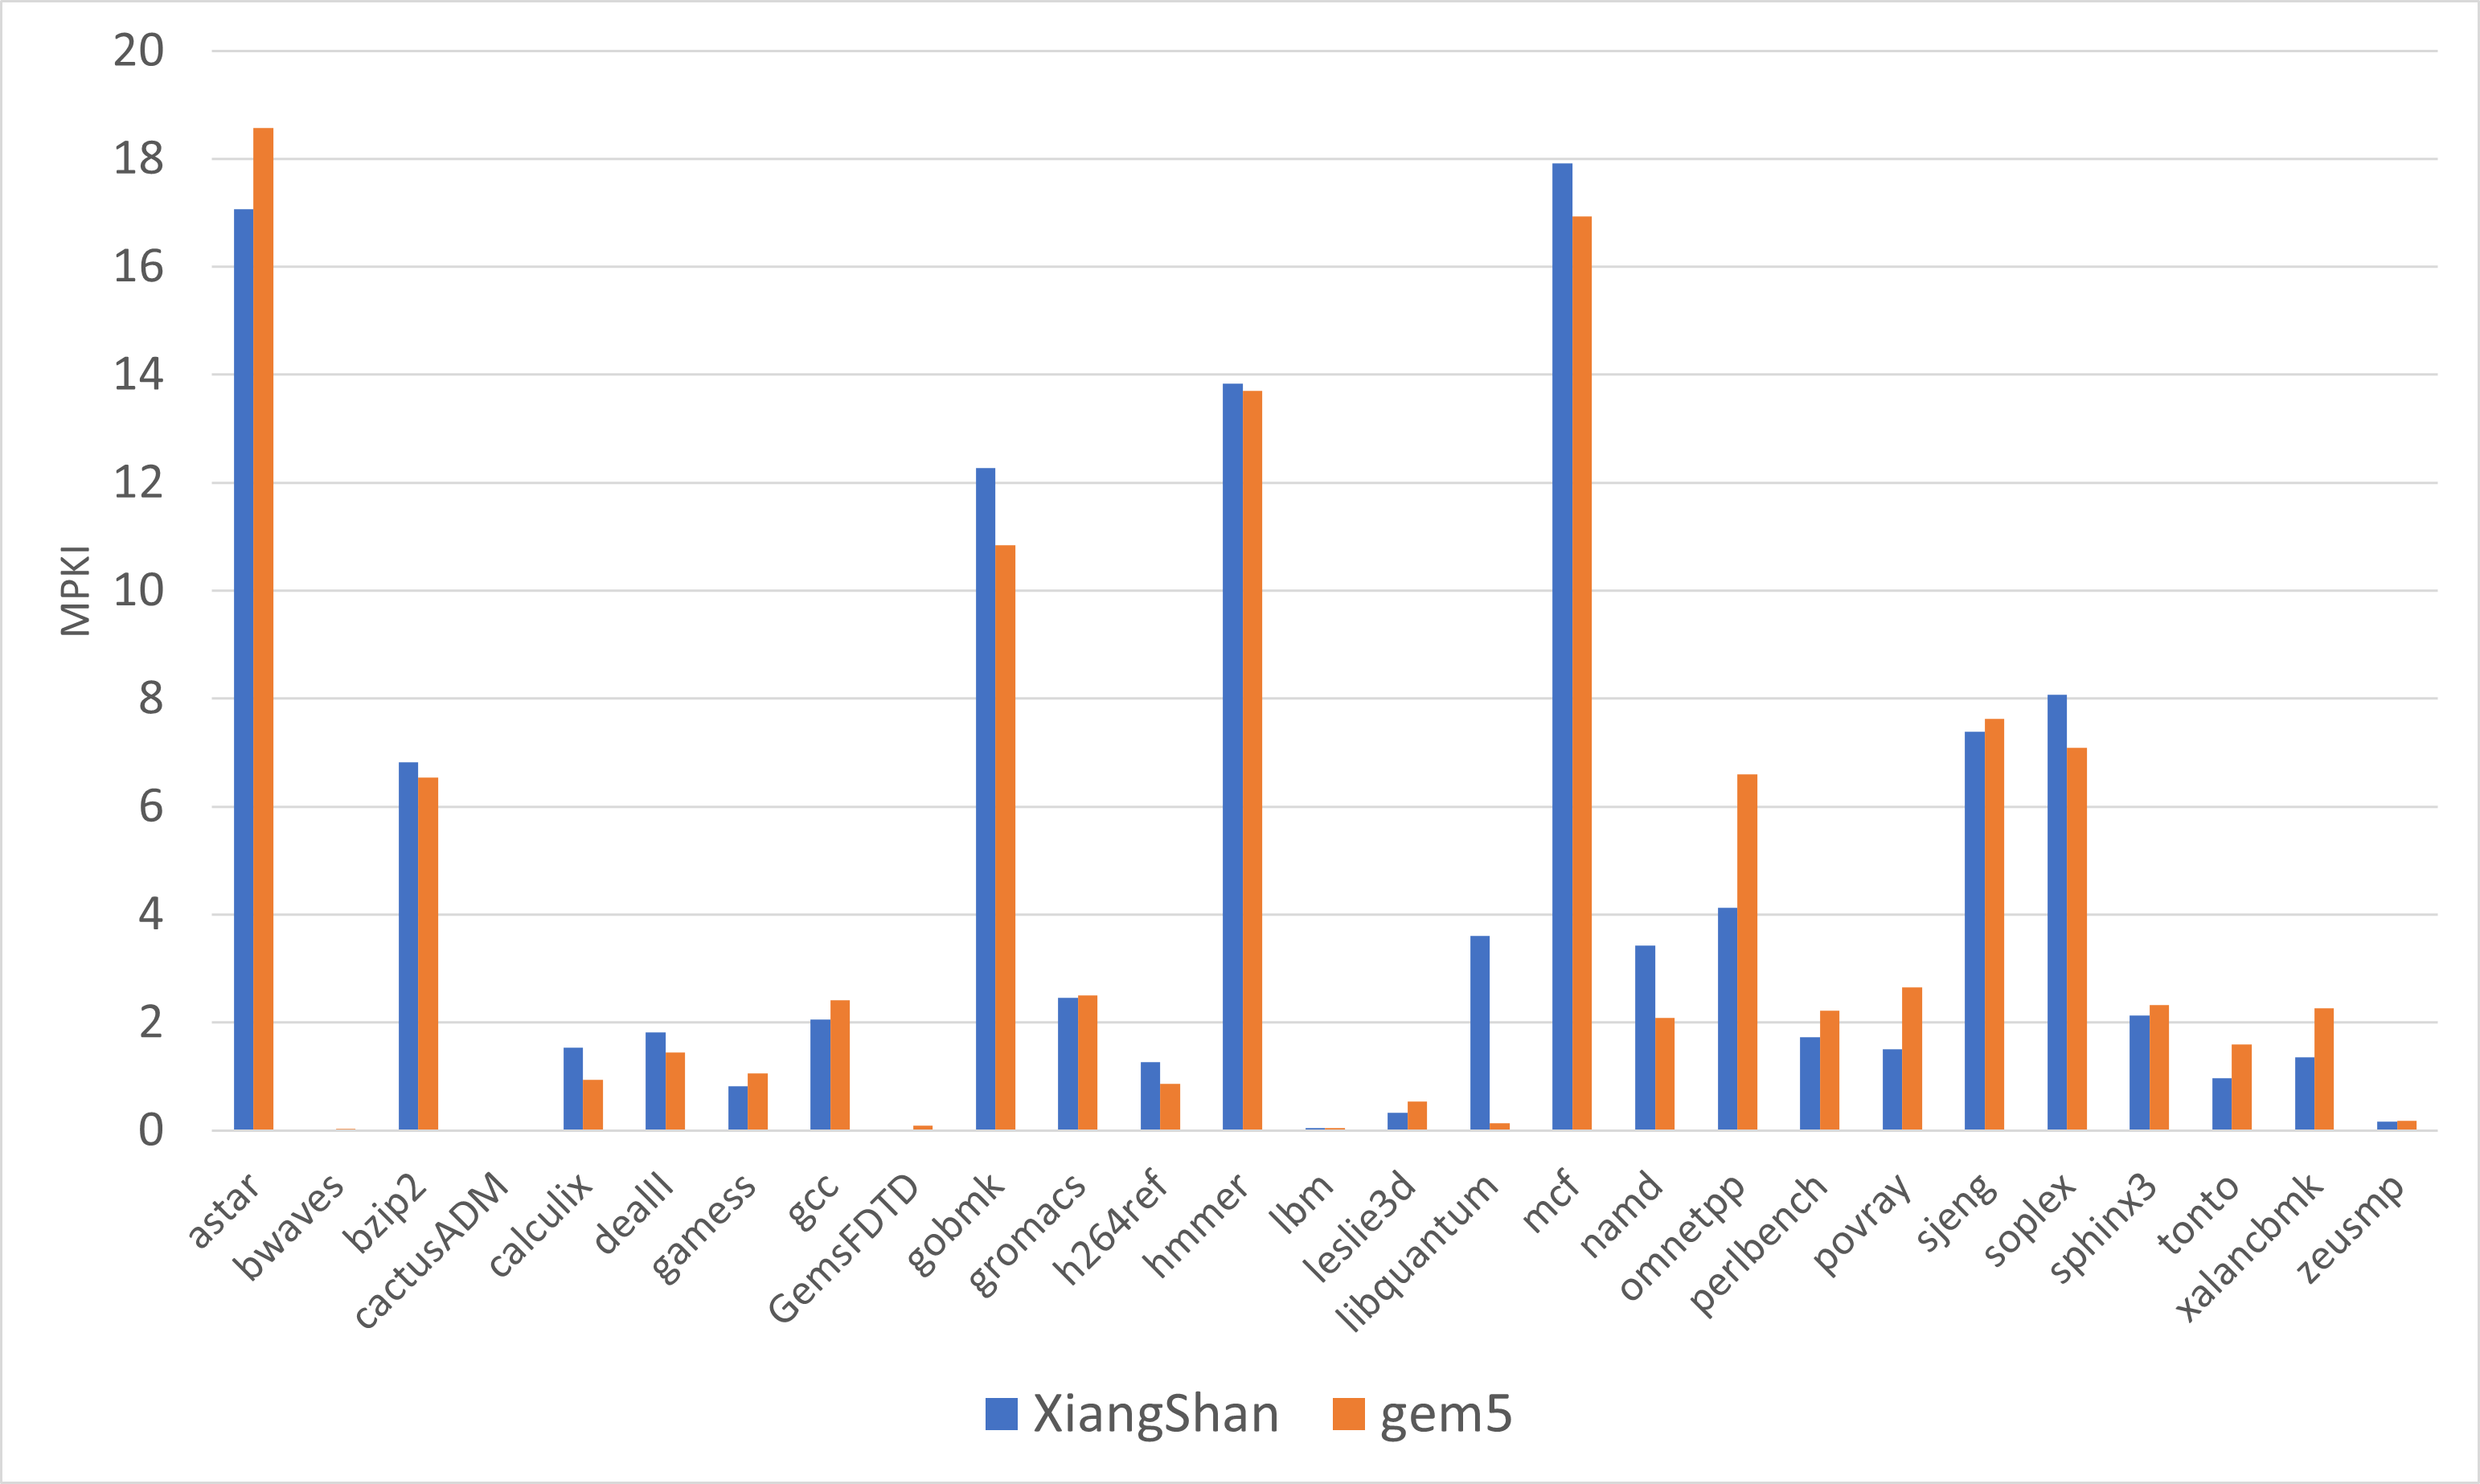
\includegraphics[width=0.9\textwidth]{xs-gem5-mpki}
    \caption{同配置下香山分支方向预测和Gem5分支预测MPKI对比}
    \label{fig:xs-gem5-mpki}
\end{figure}
主预测器决定了分支指令最终的预测结果,其误预测率是分支预测部件总体性能的关键一环。出于项目进度的考虑,我们并未对其进行形式化验证,而是在Gem5实现相同规格和算法的条件分支方向预测器,并将两者运行相同测试集的误预测率进行对比。得到的结果如图\ref{fig:xs-gem5-mpki}所示。可以看到两者在大部分测试集上预测性能近似,在个别测试集例如libquantum上预测性能差距相对较大。在所选取的测试集上,香山处理器分支预测部件主预测器的平均MPKI是4.17,同等配置下Gem5的平均MPKI是4.12。

\subsubsection*{Statistical Corrector实现效果}
\begin{figure}[!htbp]
    \begin{subfigure}{.45\textwidth}
        \centering
        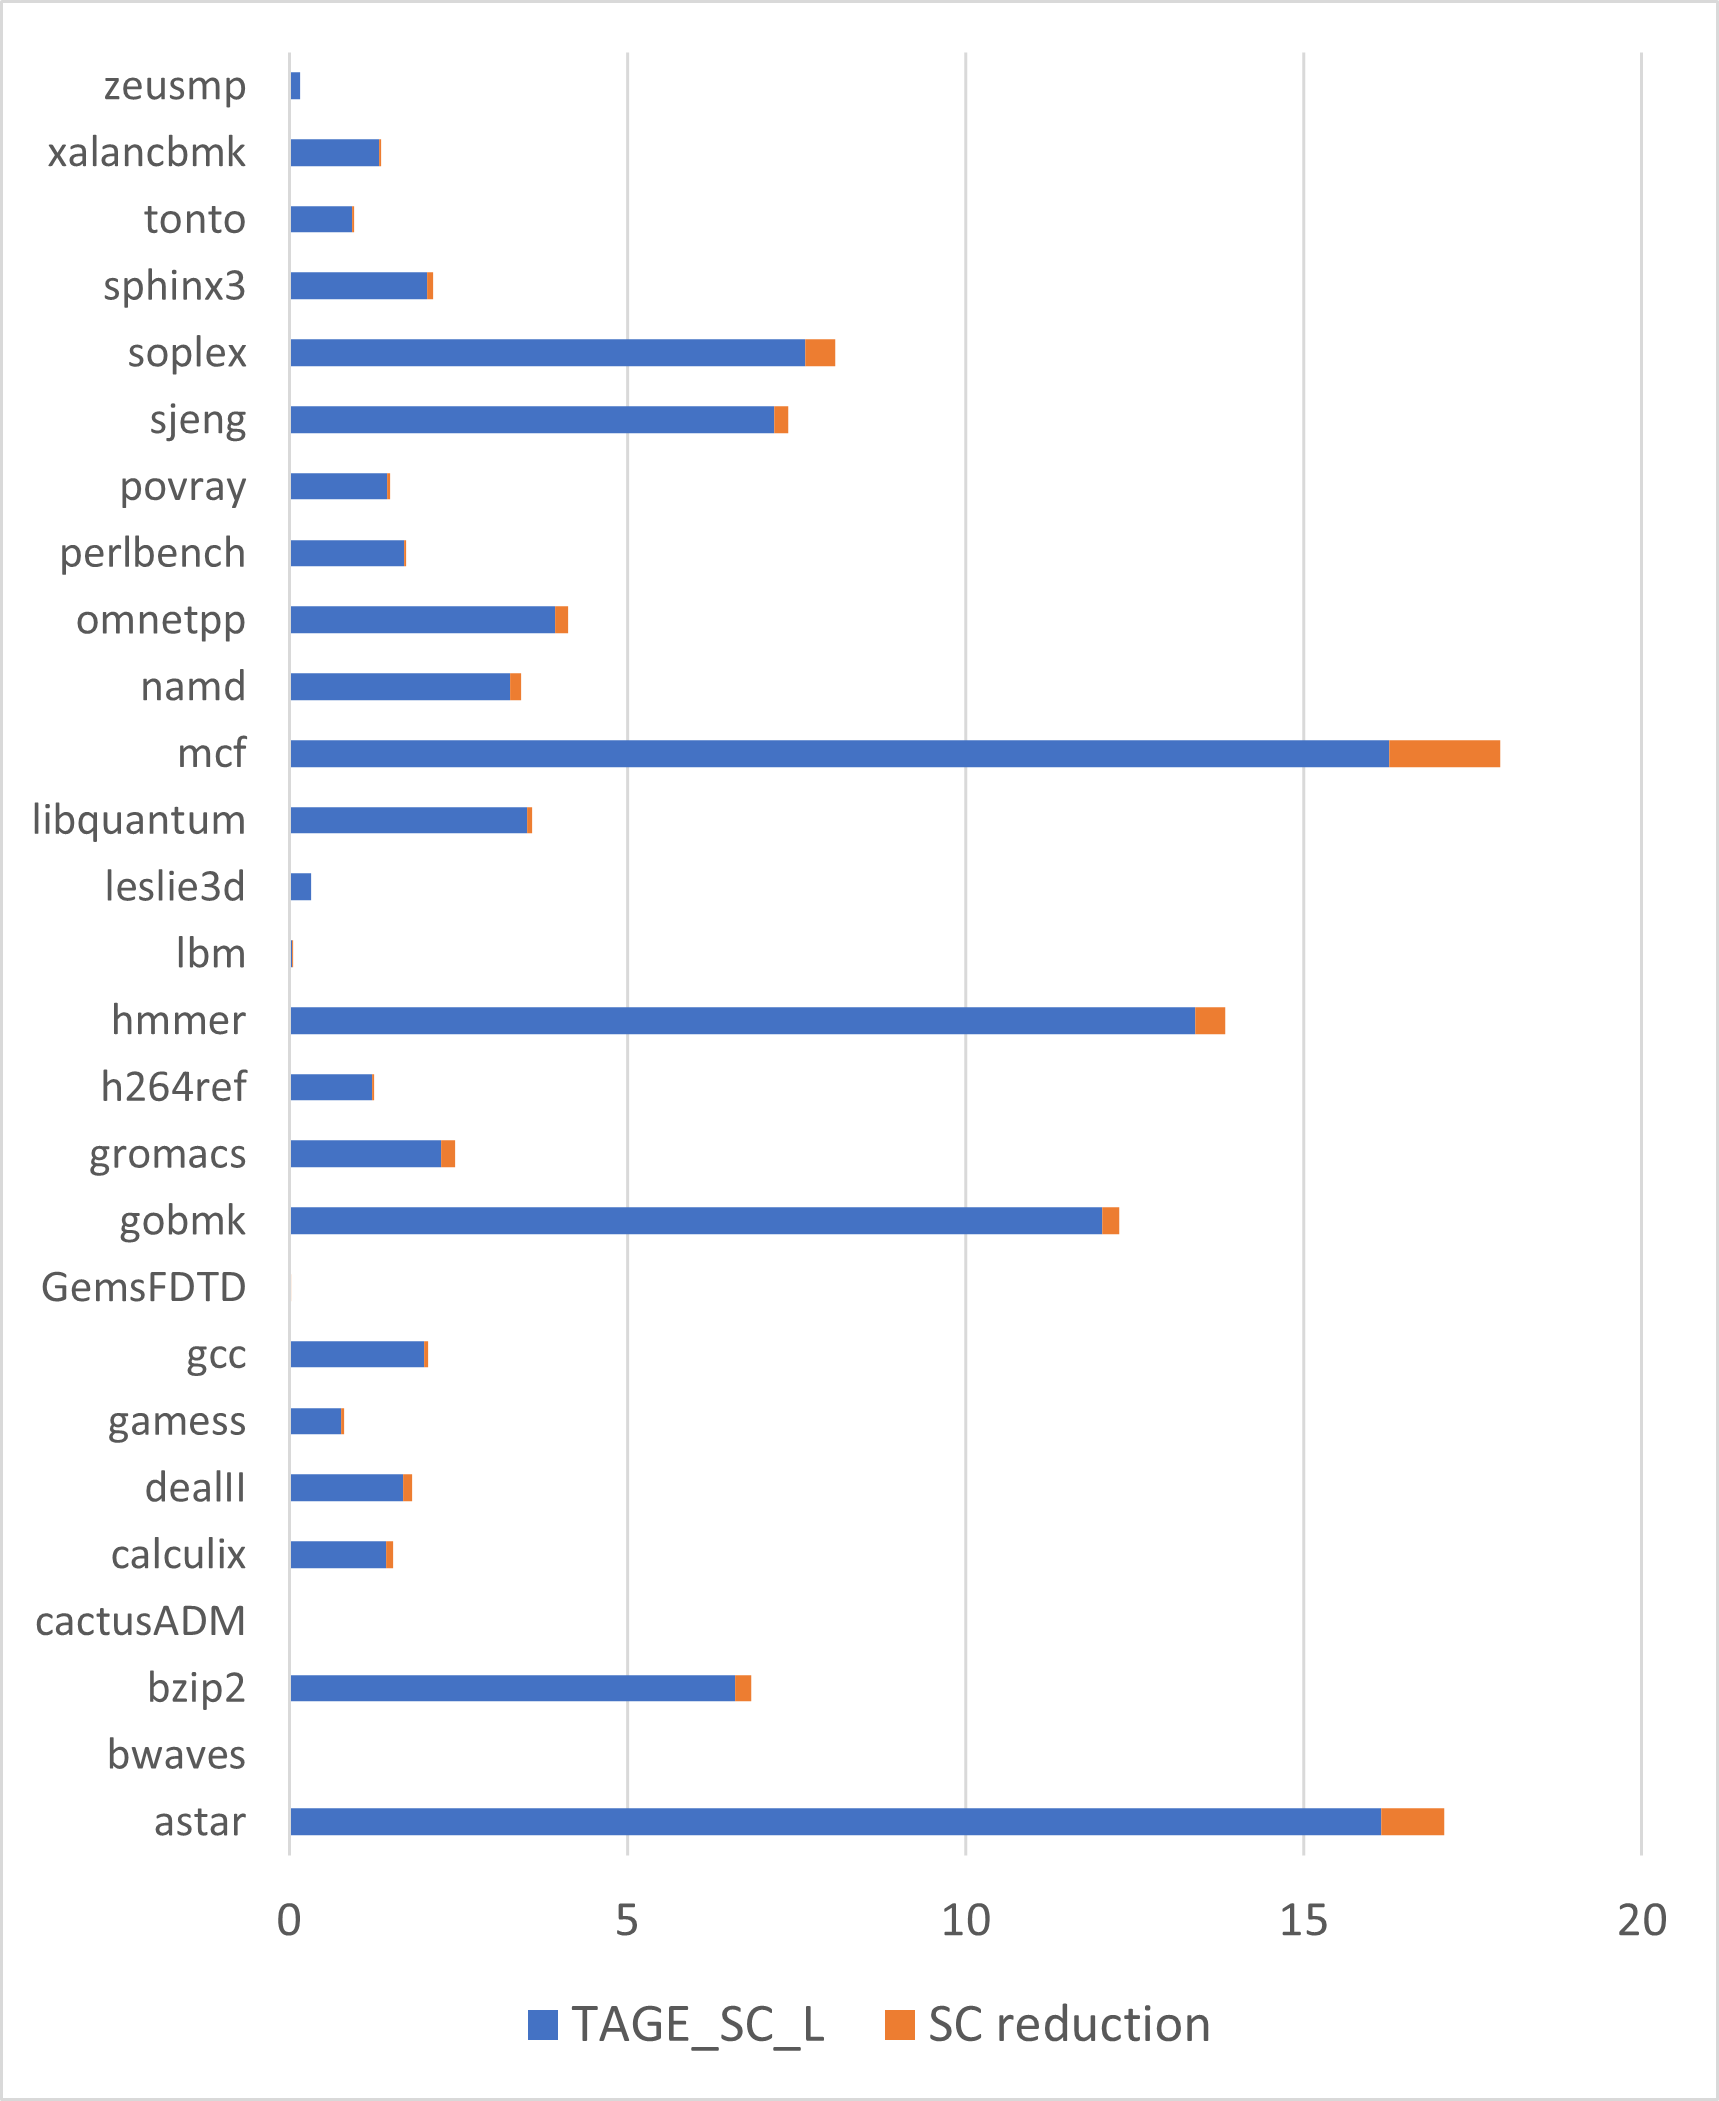
\includegraphics[width=\linewidth]{sc-mpki}
        \caption{SC降低的MPKI绝对值}
        \label{fig:sc-mpki}
    \end{subfigure}
    \begin{subfigure}{.45\textwidth}
        \centering
        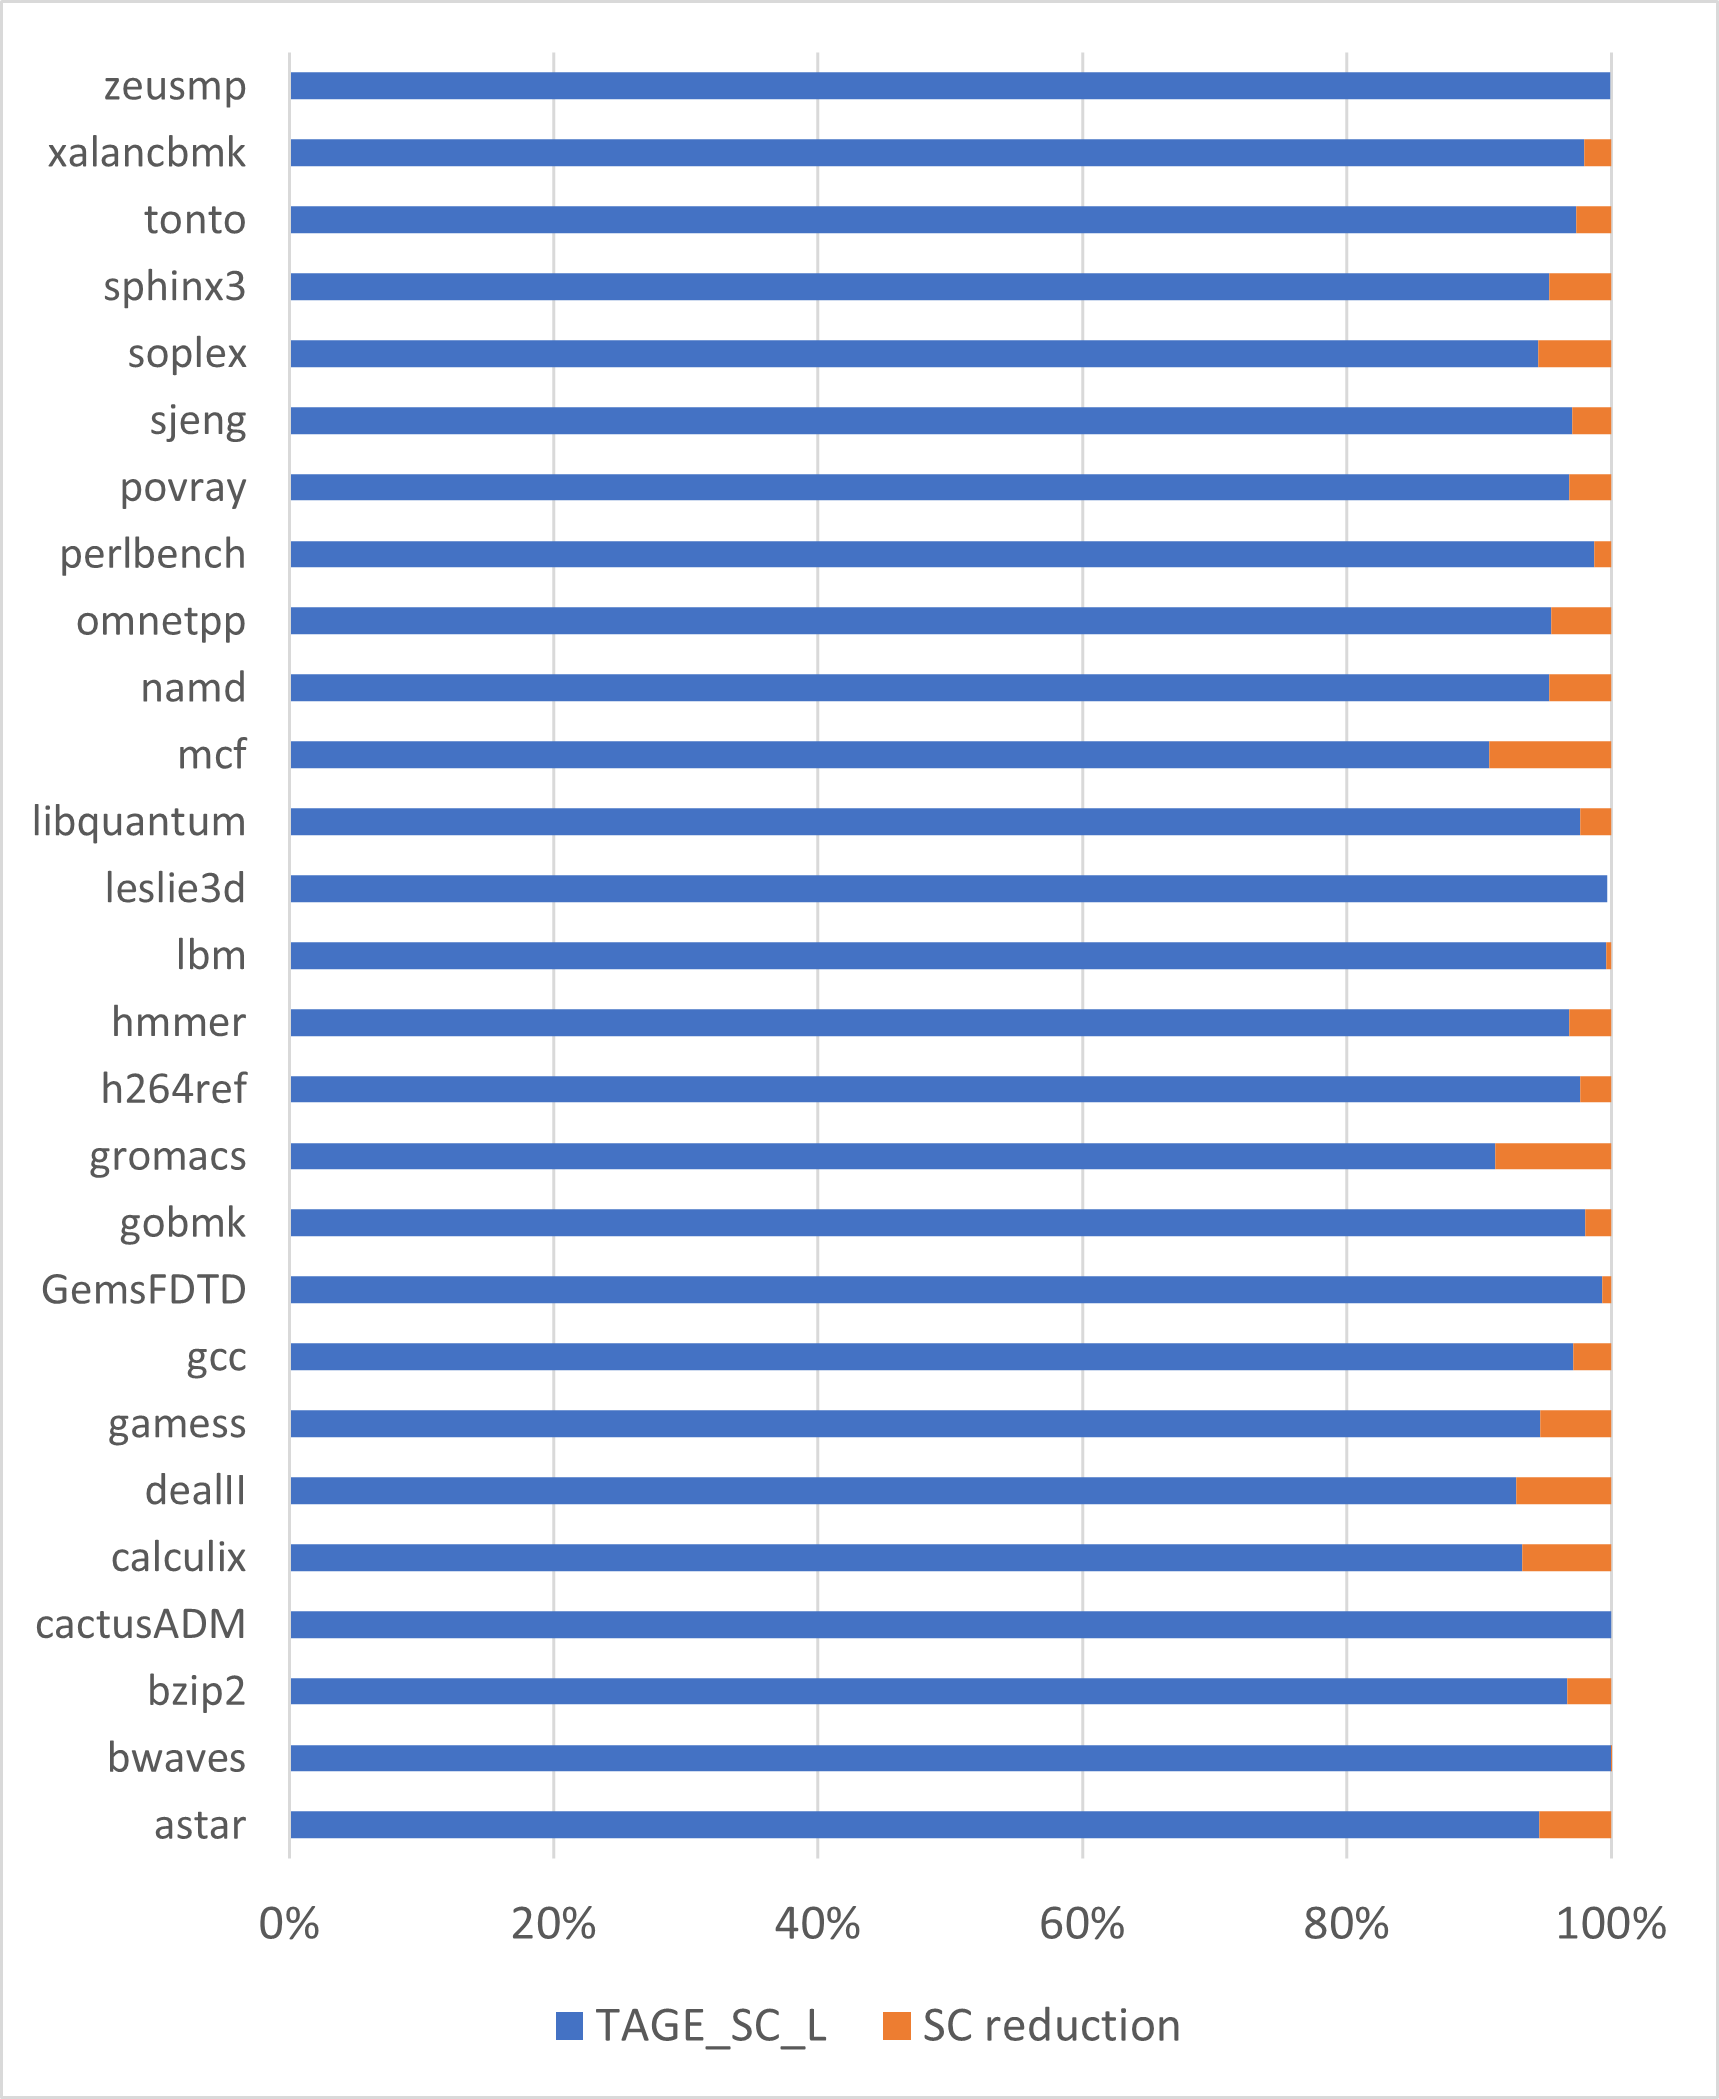
\includegraphics[width=\linewidth]{sc-mpki-rate}
        \caption{SC降低的MPKI百分比}
        \label{fig:sc-mpki-rate}
    \end{subfigure}
    \caption{Statistical Corrector对MPKI的降低}
    \label{fig:sc}
\end{figure}
我们在BOOM实现的LTAGE基础上,添加了Statistical Corrector实现。这个部件会检测某些LTAGE大概率预测错的情况进行修正,从而提升总体预测准确率。测试结果如图\ref{fig:sc},图\ref{fig:sc-mpki}中的蓝色柱形表示TAGE-SC-L的最终MPKI,橙色柱形表示在没有Statiscal Corrector的情况下会增加的MPKI;图\ref{fig:sc-mpki-rate}将图\ref{fig:sc-mpki}用百分比的形式呈现。在我们的测试集上,Statistical Corrector平均可以降低3\%左右的MPKI,可以看出该实现是有效果的。

\subsubsection*{三级预测各自对分支指令的预测准确率比较}
\begin{figure}[!htbp]
    \centering
    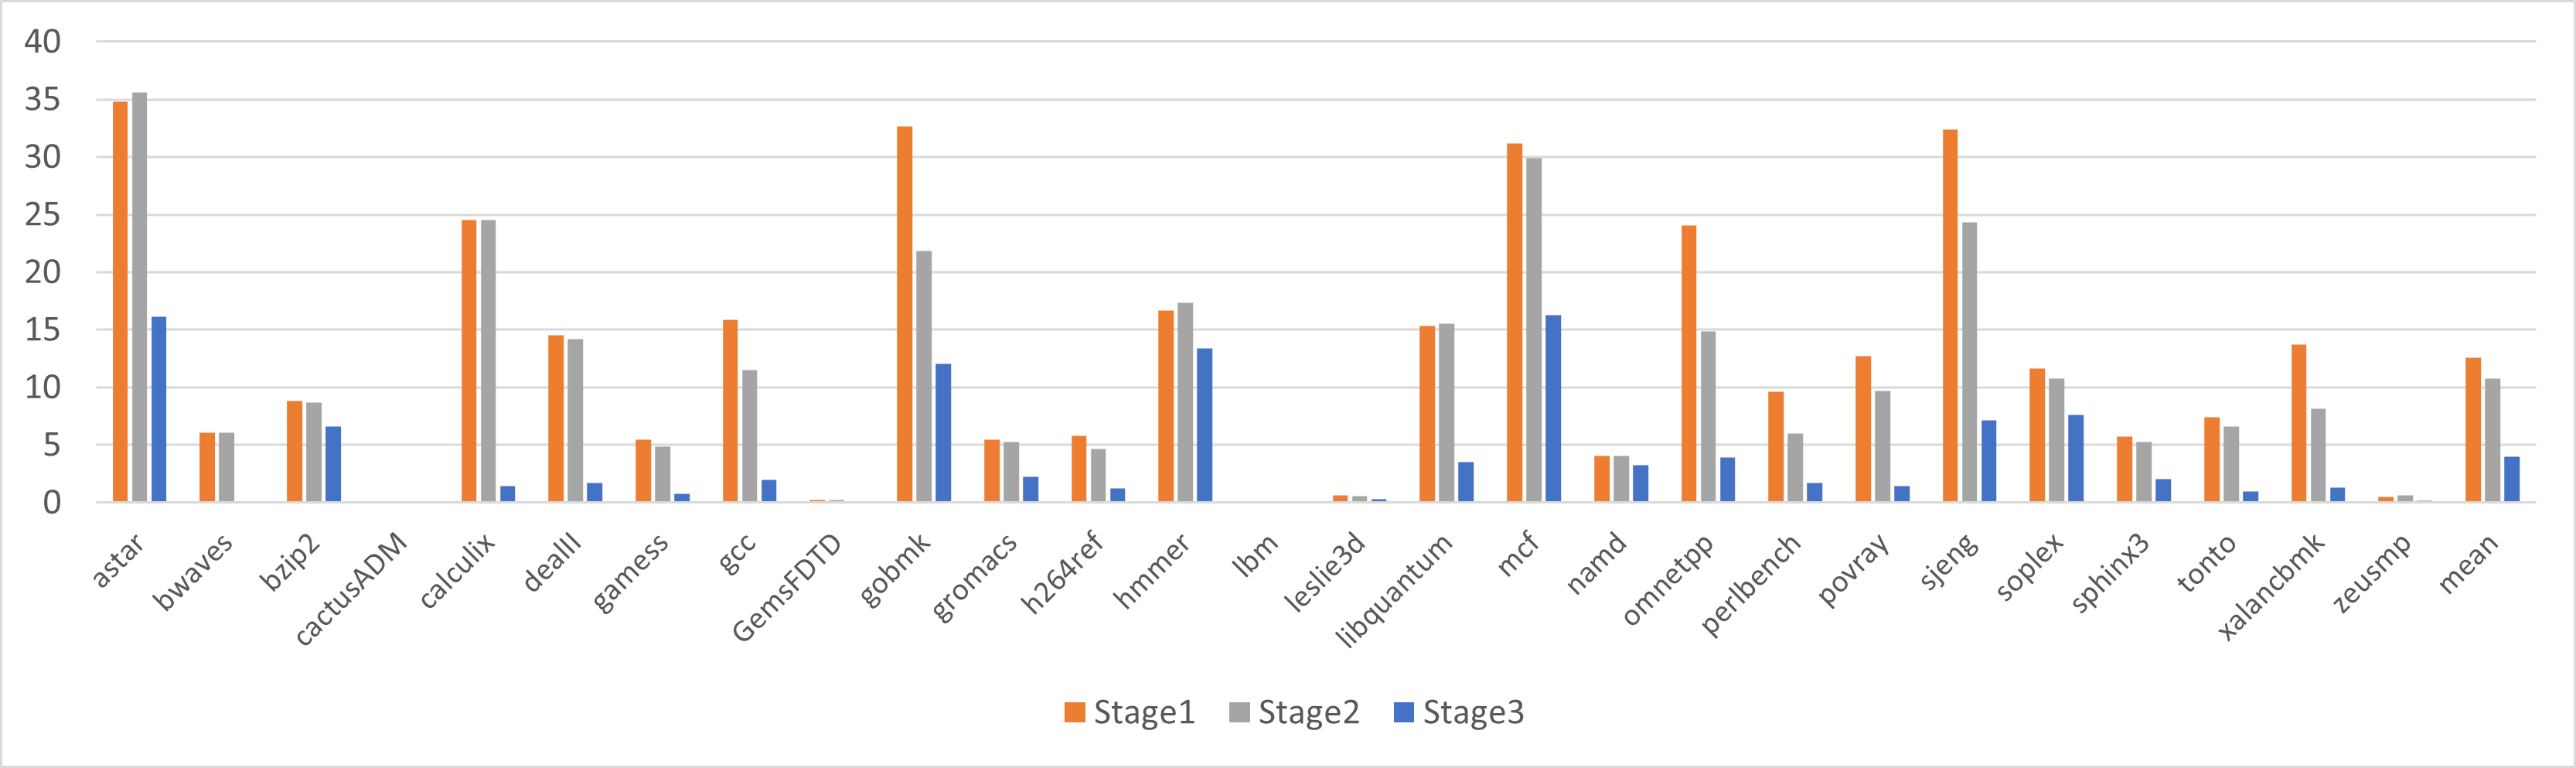
\includegraphics[width=\textwidth]{overriding-mpki}
    \caption{香山处理器分支预测各流水级的MPKI对比}
    \label{fig:overriding-mpki}
\end{figure}
\begin{table}[!htbp]
    \centering
    \footnotesize% fontsize
    \setlength{\tabcolsep}{4pt}% column separation
    \renewcommand{\arraystretch}{1.2}%row space 
    \begin{tabular}{cccc}
        %\cline{2-9}% partial hline from column i to column j
        \hline
        预测流水级 & Stage1 & Stage2 & Stage3 \\
        \hline
        MPKI      & 12.73  & 10.98  & 3.90 \\
        \hline
    \end{tabular}
    \caption{各级分支预测MPKI}
    \label{tab:overriding}
\end{table}
三级覆盖预测的假设中,后面流水级的预测一定比前面的流水级准,所以可以用后面的预测覆盖前面的预测。相邻两级的误预测率差距越大,后一级带来的性能收益越大。我们对各级的分支误预测情况进行了分别统计,得到数据如图\ref{fig:overriding-mpki}和表\ref{tab:overriding}。图\ref{fig:overriding-mpki}中“mean”的那一列表示所有测试项的平均值。可以看到,这些测试项之中主要存在几类情况:
\begin{enumerate}
    \item[\textbf{情况1}] 第一、二级MPKI差距不大,第三级MPKI显著低于其它两级,例如astar、mcf等;\label{overriding:cond1}
    \item[\textbf{情况2}] 第一、二级MPKI差距不大,第三级MPKI略低于其它两级,例如hmmer,bzip2等;\label{overriding:cond2}
    \item[\textbf{情况3}] 相邻流水级MPKI差距均相对较大,三级MPKI呈阶梯状分布,例如gobmk,omnetpp等;\label{overriding:cond3}
\end{enumerate}

第一级的条件分支预测依靠MicroBTB和两位饱和计数器;第二级的条件分支预测依靠BTB和两位饱和计数器。两级的预测机制并没有本质差别,区别仅在于使用的表项数目的多少。第一级可以预测最多256个目标地址和分支方向;第二级可以预测2048个目标地址和4096个分支方向。如果两级之间的预测差距不大,表明该测试的静态分支指令数目不多,且映射冲突不多;反之,则意味着测试中有很多静态指令或有着较多的映射冲突。情况1和情况2均属于前者。在全部的28个测试子项中,有21个子项有着这样的特性。因此第二级预测,目前在分支预测部件中起到的性能收益是相对较小的。后续可以在该级引入一个预测延迟为两拍的分支方向预测器,以提升该流水级对分支指令的预测性能。

图中还存在个别测试项中第二级误预测率略大于第一级的情况,例如astar和hmmer,这和我们的预期不符。如果实现符合设计的话,可能的原因是因为BTB存储的低位位数小于MicroBTB。出于时序考虑,我们在MicroBTB和BTB中仅存储分支指令目标地址的低位,在预测时用PC的高位与读出的低位拼接得到目标地址。在目标地址的高位和分支指令的PC不同时,会发生地址预测错误。MicroBTB存储了20位目标地址低位,而BTB只存储了13位目标地址低位。在RISC-V指令集中,分支指令的目标地址用该指令的PC与13位有符号偏移相加得到。对于目标地址的某一位来说,高位与原指令PC对应位不同的概率永远低于低位。这意味着,存储更少位地址的BTB在预测时更容易预测错目标地址。BTB的项数较多,存储开销已经较大,如果要存储更多的地址位数,会导致面积进一步增大。因此该问题的解决还需要进行进一步的考虑和评估。

最后一级预测有着最强的分支方向预测器,和预译码带来的准确的分支目标地址,因此带来了显著更低的MPKI。该级预测在多级覆盖预测的语境下是符合设计初衷的。

后续可以对前两级误预测做进一步的分类,区分误预测的原因究竟是因为方向预测错误还是目标地址缺失,从而指导进一步的优化。